\documentclass[12pt,letterpaper]{article}
\usepackage{graphicx,textcomp}
\usepackage{natbib}
\usepackage{setspace}
\usepackage{fullpage}
\usepackage{color}
\usepackage[reqno]{amsmath}
\usepackage{amsthm}
\usepackage{fancyvrb}
\usepackage{amssymb,enumerate}
\usepackage[all]{xy}
\usepackage{endnotes}
\usepackage{lscape}
\newtheorem{com}{Comment}
\usepackage{float}
\usepackage{hyperref}
\newtheorem{lem} {Lemma}
\newtheorem{prop}{Proposition}
\newtheorem{thm}{Theorem}
\newtheorem{defn}{Definition}
\newtheorem{cor}{Corollary}
\newtheorem{obs}{Observation}
\usepackage[compact]{titlesec}
\usepackage{dcolumn}
\usepackage{tikz}
\usetikzlibrary{arrows}
\usepackage{multirow}
\usepackage{xcolor}
\newcolumntype{.}{D{.}{.}{-1}}
\newcolumntype{d}[1]{D{.}{.}{#1}}
\definecolor{light-gray}{gray}{0.65}
\usepackage{url}
\usepackage{listings}
\usepackage{color}

\definecolor{codegreen}{rgb}{0,0.6,0}
\definecolor{codegray}{rgb}{0.5,0.5,0.5}
\definecolor{codepurple}{rgb}{0.58,0,0.82}
\definecolor{backcolour}{rgb}{0.95,0.95,0.92}



\lstdefinestyle{mystyle}{
	backgroundcolor=\color{backcolour},   
	commentstyle=\color{codegreen},
	keywordstyle=\color{magenta},
	numberstyle=\tiny\color{codegray},
	stringstyle=\color{codepurple},
	basicstyle=\footnotesize,
	breakatwhitespace=false,         
	breaklines=true,                 
	captionpos=b,                    
	keepspaces=true,                 
	numbers=left,                    
	numbersep=5pt,                  
	showspaces=false,                
	showstringspaces=false,
	showtabs=false,                  
	tabsize=2
}
\lstset{style=mystyle}
\newcommand{\Sref}[1]{Section~\ref{#1}}
\newtheorem{hyp}{Hypothesis}

\title{Problem Set 4}
\date{Due: April 12, 2024}
\author{Applied Stats II}


\begin{document}
	\maketitle
	\section*{Instructions}
	\begin{itemize}
	\item Please show your work! You may lose points by simply writing in the answer. If the problem requires you to execute commands in \texttt{R}, please include the code you used to get your answers. Please also include the \texttt{.R} file that contains your code. If you are not sure if work needs to be shown for a particular problem, please ask.
	\item Your homework should be submitted electronically on GitHub in \texttt{.pdf} form.
	\item This problem set is due before 23:59 on Friday April 12, 2024. No late assignments will be accepted.

	\end{itemize}

	\vspace{.25cm}
\section*{Question 1}
\vspace{.25cm}
\noindent We're interested in modeling the historical causes of child mortality. We have data from 26855 children born in Skellefteå, Sweden from 1850 to 1884. Using the "child" dataset in the \texttt{eha} library, fit a Cox Proportional Hazard model using mother's age and infant's gender as covariates. Present and interpret the output.

\lstinputlisting[language=R, firstline=1, lastline=22]{PS4.R}
\begin{table}[htbp]
    \centering
    \caption{head(child)}
    \label{tab:your_table_label}
    \begin{tabular}{cccccccccc} % Adjust the number of 'c's based on the number of columns in your data frame
        \hline
        id & m.id & sex & socBranch & birthdate & enter & exit & event & illeg & m.age \\
        \hline
        3 & 9 & male & farming & 1853-05-23 & 0 & 15.000 & 0 & no & 35.009 \\
        42 & 150 & male & farming & 1853-07-19 & 0 & 15.000 & 0 & no & 30.609 \\
        47 & 158 & male & worker & 1861-11-17 & 0 & 15.000 & 0 & no & 29.320 \\
        54 & 178 & male & farming & 1872-11-16 & 0 & 15.000 & 0 & no & 41.183 \\
        78 & 263 & female & worker & 1855-07-19 & 0 & 0.559 & 1 & no & 42.138 \\
        102 & 342 & male & farming & 1855-09-29 & 0 & 0.315 & 1 & no & 32.931 \\
        \hline
    \end{tabular}
\end{table}
\lstinputlisting[language=R, firstline=31, lastline=32]{PS4.R}
\begin{table}[htbp]
    \centering
    \caption{str(child)} 
    \label{tab:your_table_label}
    \begin{tabular}{cccccccccc} 
        \hline
        id & m.id & sex & socBranch & birthdate & enter & exit & event & illeg & m.age \\
        \hline
        9 & 246606 & male & farming & 1853-05-23 & 0 & 15.000 & 0 & no & 35.009 \\
        150 & 377744 & male & farming & 1853-07-19 & 0 & 15.000 & 0 & no & 30.609 \\
        158 & 118277 & male & worker & 1861-11-17 & 0 & 15.000 & 0 & no & 29.320 \\
        178 & 715337 & male & farming & 1872-11-16 & 0 & 15.000 & 0 & no & 41.183 \\
        263 & 978617 & female & worker & 1855-07-19 & 0 & 0.559 & 1 & no & 42.138 \\
        342 & 282943 & male & farming & 1855-09-29 & 0 & 0.315 & 1 & no & 32.931 \\
        363 & 341341 & male & farming & 1858-07-25 & 0 & 15.000 & 0 & no & 38.670 \\
        393 & 840879 & male & farming & 1871-04-29 & 0 & 15.000 & 0 & no & 35.059 \\
        408 & 586140 & female & farming & 1859-07-06 & 0 & 15.000 & 0 & no & 33.515 \\
        486 & 564736 & female & farming & 1862-08-16 & 0 & 15.000 & 0 & yes & 29.525 \\
        \hline
    \end{tabular}
\end{table}
\lstinputlisting[language=R, firstline=45, lastline=46]{PS4.R}
A data frame with 26855 children born 1850-1884.\\
\\
id: An identification number.\\
m.id: Mother's id.\\
sex: Sex.\\
socBranch: Working branch of family (father).\\
birthdate: Birthdate.\\
enter: Start age of follow-up, always zero.\\
exit: Age of departure, either by death or emigration.\\
event: Type of departure, death = 1, right censoring = 0.\\
illeg: Born out of marriage ("illegitimate")?\\
m.age: Mother's age.\\

\lstinputlisting[language=R, firstline=62, lastline=63]{PS4.R}
[1] 26574    10\\
The dataset 'child' has 26574 rows and 10 columns.\\
\lstinputlisting[language=R, firstline=67, lastline=68]{PS4.R}
\begin{verbatim}
Min. 1st Qu.  Median    Mean 3rd Qu.    Max. 
15.83   27.18   31.79   32.03   36.74   50.86 
\end{verbatim}

\lstinputlisting[language=R, firstline=72, lastline=76]{PS4.R}
\begin{verbatim}
Covariate             Mean       Coef     Rel.Risk   S.E.    LR p
sex                                                          0.002 
            male      0.510     0         1 (reference)
          female      0.490    -0.082     0.921     0.027
m.age                32.010     0.008     1.008     0.002    0.000 

Events                    5616 
Total time at risk        325030 
Max. log. likelihood      -56503 
LR test statistic         22.52 
Degrees of freedom        2 
Overall p-value           1.28921e-05
\end{verbatim}
\\\\
In this case, we observed the following:\\\\
The sex of the infants significantly affects their survival rate. The relative risk (or hazard) ratio for female infants compared to male infants is 0.921, indicating a decrease in relative risk by 8.1\%. This suggests that female infants are more likely to survive.\\\\
Mother's age also influences the infant's survival rate. For each unit increase in age (e.g., one year), the relative risk increases by 0.8\%.\\\\
The LR test statistic is 22.52, indicating the degree of improvement in model fit after adding variables. In this case, the large value of the LR test statistic suggests a significant improvement in model fit after adding variables.\\\\
The p-value is 1.28921e-05, close to zero, indicating that the overall model fit is significant, meaning that at least one covariate has a significant impact on survival time.\\\\

\lstinputlisting[language=R, firstline=101, lastline=118]{PS4.R}

\begin{verbatim}
Call: survfit(formula = child_surv ~ 1, data = child)

time n.risk n.event survival std.err lower 95% CI upper 95% CI
    0  26574       0    1.000 0.00000        1.000        1.000
    1  24319    2161    0.919 0.00168        0.915        0.922
    2  23450     778    0.889 0.00193        0.885        0.893
    3  22766     596    0.867 0.00209        0.862        0.871
    4  22269     430    0.850 0.00220        0.846        0.854
    5  21859     365    0.836 0.00228        0.832        0.841
    6  21533     261    0.826 0.00233        0.822        0.831
    7  21266     214    0.818 0.00238        0.813        0.823
    8  21077     151    0.812 0.00241        0.807        0.817
    9  20915     117    0.808 0.00243        0.803        0.812
   10  20777     103    0.804 0.00245        0.799        0.808
   11  20655      81    0.801 0.00246        0.796        0.805
   12  20531      91    0.797 0.00248        0.792        0.802
   13  20404      89    0.794 0.00250        0.789        0.798
   14  20277      95    0.790 0.00251        0.785        0.795
   15  20141      84    0.787 0.00253        0.782        0.792
\end{verbatim}
\noindent
As time progresses, the survival rate gradually decreases.\\
For example, at the first time point (time = 0), the survival rate is 1, indicating that all individuals are alive at the starting time point;\\\\
whereas at the 15th time point, the survival rate decreases to 0.787, indicating that approximately 78.7\% of individuals are still alive at that time point.\\\\
The decline in survival rate implies an increase in mortality rate.\\\\
The survival rate gradually decreases, indicating that at each time point, more individuals experience the event (such as death), thus the mortality rate increases gradually.

\lstinputlisting[language=R, firstline=147, lastline=148]{PS4.R}
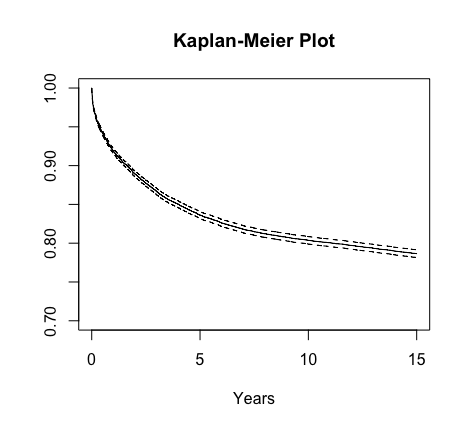
\includegraphics[width=0.99\textwidth]{Kaplan-Meier Plot_PS04.png}

\lstinputlisting[language=R, firstline=149, lastline=150]{PS4.R}
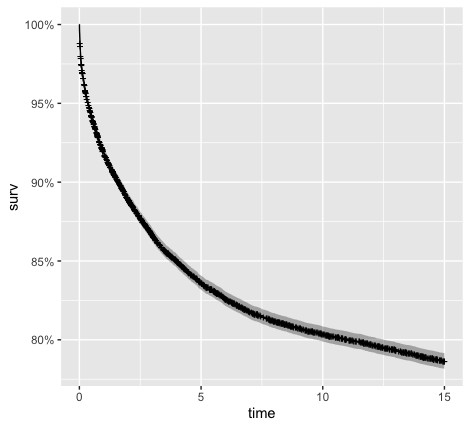
\includegraphics[width=0.99\textwidth]{autoplot(km)_PS04.png}

\lstinputlisting[language=R, firstline=152, lastline=163]{PS4.R}
\begin{verbatim}
Call:
coxph(formula = child_surv ~ sex + m.age, data = child)

  n= 26574, number of events= 5616 

               coef exp(coef)  se(coef)      z Pr(>|z|)    
sexfemale -0.082215  0.921074  0.026743 -3.074 0.002110 ** 
m.age      0.007617  1.007646  0.002128  3.580 0.000344 ***
---
Signif. codes:  0 ‘***’ 0.001 ‘**’ 0.01 ‘*’ 0.05 ‘.’ 0.1 ‘ ’ 1

          exp(coef) exp(-coef) lower .95 upper .95
sexfemale    0.9211     1.0857     0.874    0.9706
m.age        1.0076     0.9924     1.003    1.0119

Concordance= 0.519  (se = 0.004 )
Likelihood ratio test= 22.52  on 2 df,   p=1e-05
Wald test            = 22.52  on 2 df,   p=1e-05
Score (logrank) test = 22.53  on 2 df,   p=1e-05
\end{verbatim}
\\\\
Interpretation of summary statistics output:\\\\
coef: In this example, the coef for sexfemale is -0.0822, indicating a decrease in risk by -0.0822 units relative to male infants. The coef for m.age is 0.0076, suggesting that for each additional year of mother's age, the risk of death for her infant increases by 0.0076 units.\\\\
exp(coef): The exponentiated coefficients represent the relative hazard ratios for each variable, indicating changes in risk relative to the reference level.\\\\
In this example, the exp(coef) for sexfemale is 0.9211, indicating a reduction in hazard ratio by 0.9211 units compared to male infants. For m.age, exp(coef) is 1.0076, implying that relative to the reference level (which is the baseline for m.age, likely the median or mean age), the hazard ratio for infants increases by a factor of 1.0076.

\lstinputlisting[language=R, firstline=192, lastline=194]{PS4.R}
\begin{verbatim}
Single term deletions

Model:
child_surv ~ sex + m.age
       Df    AIC     LRT  Pr(>Chi)    
<none>    113011                      
sex     1 113018  9.4646 0.0020947 ** 
m.age   1 113022 12.7946 0.0003476 ***
---
Signif. codes:  0 ‘***’ 0.001 ‘**’ 0.01 ‘*’ 0.05 ‘.’ 0.1 ‘ ’ 1
\end{verbatim}
\\\\
In this output, we observe the results of the deletion tests for two explanatory variables: \\\\
sex and m.age:\\
The deletion test results for the sex variable indicate that when the sex variable is removed from the model, 
the model's Log Likelihood Ratio Test (LRT) statistic is 9.4646, with a corresponding p-value of 0.0020947.\\\\ 
This suggests that the sex variable has a significant effect in the model, indicating that gender has a significant impact on infant survival time.\\\\
The deletion test results for the m.age variable indicate that when the m.age variable is removed from the model, the model's LRT statistic is 12.7946, with a corresponding p-value of 0.0003476.\\\\ 
Similarly, this indicates that the m.age variable has a significant effect in the model, suggesting that mother's age also has a significant impact on infant survival time.\\\\
Therefore, this test result informs us that both gender and mother's age are significant explanatory variables in the model, and they both have important effects on infant survival time.

\lstinputlisting[language=R, firstline=220, lastline=221]{PS4.R}

\begin{verbatim}
================================================
                         Dependent variable:    
                     ---------------------------
                             child_surv         
------------------------------------------------
sexfemale                     -0.082***         
                               (0.027)          
                                                
m.age                         0.008***          
                               (0.002)          
                                                
------------------------------------------------
Observations                   26,574           
R2                              0.001           
Max. Possible R2                0.986           
Log Likelihood               -56,503.480        
Wald Test                22.520*** (df = 2)     
LR Test                  22.518*** (df = 2)     
Score (Logrank) Test     22.530*** (df = 2)     
================================================
Note:                *p<0.1; **p<0.05; ***p<0.01
\end{verbatim}
\\\\
The results of this Cox proportional hazards model are crucial for understanding the impact on infant survival time, particularly concerning gender and maternal age.\\\\
1. Effect of Gender (sexfemale) on Infant Survival Time:\\
 - The coefficient (Coef) is -0.082, indicating that the survival time risk for female infants decreases by 0.082 relative to male infants. This suggests that, all other factors being equal, female infants are more likely to survive.\\
- In practical terms, female infants exhibit higher survival rates compared to male infants.\\\\
2. Effect of Maternal Age (m.age) on Infant Survival Time:\\
 - The Coef is 0.008, signifying that for each additional year of maternal age, the infant's survival time risk increases by 0.008. This implies that infants born to older mothers are more likely to face mortality risks.\\\\
\lstinputlisting[language=R, firstline=255, lastline=256]{PS4.R}
[1] 0.9210739\\\\
The hazard ratio for female infants is 0.92, indicating a lower risk of mortality compared to male infants. \\
This can be interpreted as approximately 92 female infants potentially dying for every 100 male infants. \\
This suggests that the risk for female infants is reduced by approximately 9.21\% compared to male infants.\\


\lstinputlisting[language=R, firstline=264, lastline=266]{PS4.R}
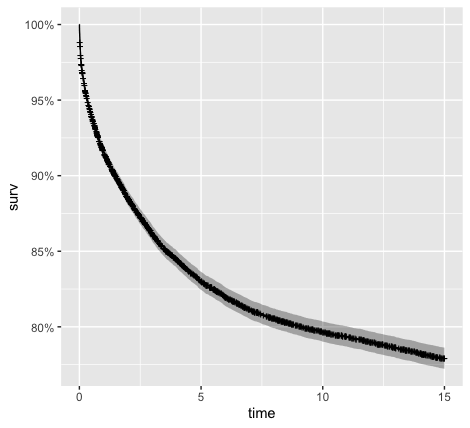
\includegraphics[width=0.99\textwidth]{autoplot(cox_fit)_PS04.png}
\lstinputlisting[language=R, firstline=269, lastline=271]{PS4.R}
[1] 31.789\\
setting the median age as the reference line\\

\lstinputlisting[language=R, firstline=276, lastline=299]{PS4.R}
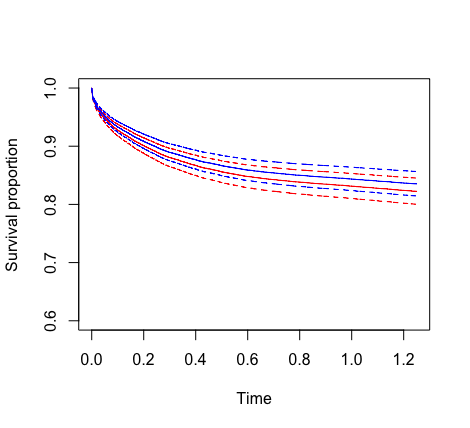
\includegraphics[width=0.99\textwidth]{Survival proportion_PS04.png}
\lstinputlisting[language=R, firstline=302, lastline=308]{PS4.R}
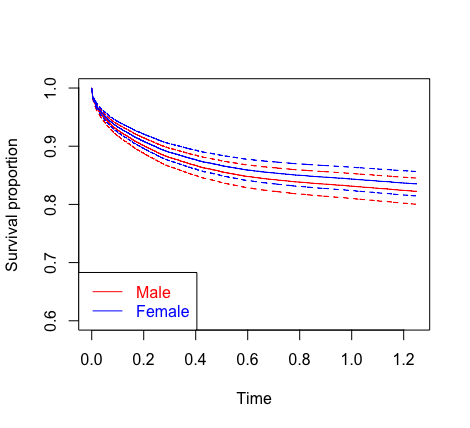
\includegraphics[width=0.99\textwidth]{Survival proportion(with bottomleft)_PS04.png}

\lstinputlisting[language=R, firstline=312, lastline=318]{PS4.R}
\begin{verbatim}
Call:
coxph(formula = child_surv ~ sex * m.age, data = child)

  n= 26574, number of events= 5616 

                     coef exp(coef)  se(coef)      z Pr(>|z|)  
sexfemale       -0.127105  0.880641  0.140304 -0.906   0.3650  
m.age            0.006963  1.006987  0.002925  2.380   0.0173 *
sexfemale:m.age  0.001389  1.001390  0.004263  0.326   0.7445  
---
Signif. codes:  0 ‘***’ 0.001 ‘**’ 0.01 ‘*’ 0.05 ‘.’ 0.1 ‘ ’ 1

                exp(coef) exp(-coef) lower .95 upper .95
sexfemale          0.8806     1.1355    0.6689     1.159
m.age              1.0070     0.9931    1.0012     1.013
sexfemale:m.age    1.0014     0.9986    0.9931     1.010

Concordance= 0.519  (se = 0.004 )
Likelihood ratio test= 22.62  on 3 df,   p=5e-05
Wald test            = 22.53  on 3 df,   p=5e-05
Score (logrank) test = 22.56  on 3 df,   p=5e-05
\end{verbatim}
\\\\
An interaction term has been added here to examine the joint effect of mother's age and infant gender. \\\\
Specifically:\\
This Cox proportional hazards model considers the interaction between infant gender and mother's age on infant survival time.\\
`sexfemale` and `m.age` represent the two main explanatory variables in the model, which are gender and mother's age, respectively.\\
For `sexfemale`, the coefficient is -0.127105, indicating that female infants have a lower risk compared to male infants, but the coefficient is not significant (p = 0.365).\\
Whereas for `m.age`, the coefficient is 0.006963, indicating that for each additional year of mother's age, the infant's risk increases by 0.006963.\\
This coefficient is statistically significant (p = 0.0173), suggesting that mother's age has a certain impact on infant survival time.\\
`sexfemale:m.age` is the coefficient for the interaction term between gender and mother's age, which is 0.001389, but this coefficient is not significant (p = 0.7445).\\
This indicates that the interaction between gender and mother's age does not significantly affect infant survival time when considering both factors.\\\\
The statistical test results of the model show that the p-values for Likelihood ratio test, Wald test, and Score (logrank) test are all less than 0.05, indicating that the overall model is significant, and at least one variable has a significant effect on infant survival time.\\
\lstinputlisting[language=R, firstline=357, lastline=358]{PS4.R}
\begin{verbatim}
Single term deletions

Model:
child_surv ~ sex * m.age
          Df    AIC     LRT Pr(>Chi)
<none>       113013                 
sex:m.age  1 113011 0.10623   0.7445
\end{verbatim}
\\\\\\
The `drop1()` function is used here to perform a chi-square test of model fitting, which aims to systematically remove each explanatory variable from the model and compare the difference between the reduced model and the full model.\\\\
The results here indicate that after removing the interaction term `sex:m.age`, there is no significant change in the model fit (p = 0.7445), meaning that removing this interaction term does not significantly affect the difference between the reduced model and the full model.\\\\
In other words, considering the interaction between mother's age and infant gender in the model does not significantly improve the explanatory power for survival time.\\

\lstinputlisting[language=R, firstline=375, lastline=376]{PS4.R}
\begin{verbatim}
================================================
                         Dependent variable:    
                     ---------------------------
                             child_surv         
------------------------------------------------
sexfemale                      -0.127           
                               (0.140)          
                                                
m.age                          0.007**          
                               (0.003)          
                                                
sexfemale:m.age                 0.001           
                               (0.004)          
                                                
------------------------------------------------
Observations                   26,574           
R2                              0.001           
Max. Possible R2                0.986           
Log Likelihood               -56,503.430        
Wald Test                22.530*** (df = 3)     
LR Test                  22.624*** (df = 3)     
Score (Logrank) Test     22.562*** (df = 3)     
================================================
Note:                *p<0.1; **p<0.05; ***p<0.01
\end{verbatim}
\\\\\\\\
The output presents the results of the Cox proportional hazards model in tabular form. \\\\
Explain:\\\\
sexfemale: This is the coefficient for gender, -0.127, but not significant with a p-value of 0.365. This indicates that the change in risk for female infants compared to male infants is -0.127, but this change is not significant.\\\\
m.age: This is the coefficient for mother's age, 0.007, and significant with a p-value of 0.0173. This means that for every one year increase in mother's age, the change in risk for infants is 0.007.\\\\
sexfemale:m.age: This is the coefficient for the interaction between gender and mother's age, 0.001, and not significant with a p-value of 0.7445. This suggests that the interaction between gender and mother's age is not significant in this model.\\\\
Overall, the model fit is not ideal, with an R² of only 0.001, indicating that the model does not explain much of the variation in the data.\\\\
\\\\
Summary:\\\\
In this case, we used the Cox proportional hazards model to study the survival time of infants born in the Skellefte region of Sweden from 1850 to 1884, and investigated the effects of mother's age and infant gender on infant survival time.\\\\
Firstly, we found that gender has a significant impact on survival time. Female infants have a survival time risk reduction of approximately 8.21\% compared to male infants. This suggests that, all else being equal, female infants are more likely to survive.\\\\
Secondly, mother's age also has a significant impact on infant survival time. For every one year increase in mother's age relative to the median age (approximately 31.789 years), the infant's survival time risk increases by approximately 0.76\%. This implies that infants born to older mothers are more likely to face a risk of death.\\\\
In other words, for every one year decrease in mother's age relative to the median age (approximately 31.789 years), the infant's survival time risk decreases by approximately 0.76\%. This suggests that infants born to younger mothers are more likely to enjoy longer survival times.\\\\
Additionally, we also explored the interaction between infant gender and mother's age on infant survival time. The results showed that, after considering gender and mother's age, the interaction between them did not significantly affect infant survival time.\\\\



\end{document}